Interleaving of the stages of multiple jobs is our key concept for enabling large-scale autotuning. \cite{Ma.2005} uses a design-time scheduler to create a program with good concurrency. We need to dynamically schedule incoming jobs, so the schedule cannot be predetermined. We need an additional component in the autotuning architecture that orchestrates running jobs. In this chapter, we describe the design and implementation of our central scheduler that controls stage execution.

\section{Design}
Our scheduler possesses the two features that have been determined to be imperative for optimal large-scale autotuning:
\begin{itemize}
	\item Computation resources are shared between jobs. This facilitates good resource utilization since the idle time of one job can be leveraged to execute another job. This is called \textit{interleaving} and saves hardware and costs as a result. However, stage dependencies of a single job must be maintained.
	\item Interference between jobs is prevented. This guarantees that inference performance and autotuning time are as good as possible. The scheduler needs to check if the resource that will be used by the next stage is free before execution. This might necessitate the postponing of stage executions if the stage is ready before the resource becomes free.
\end{itemize}
These two features not only make it match the optimal solution, but also do they solve the problem of bad resource utilization of single-job autotuning by leveraging that shortcoming.

\begin{figure}[h]
	\centering
	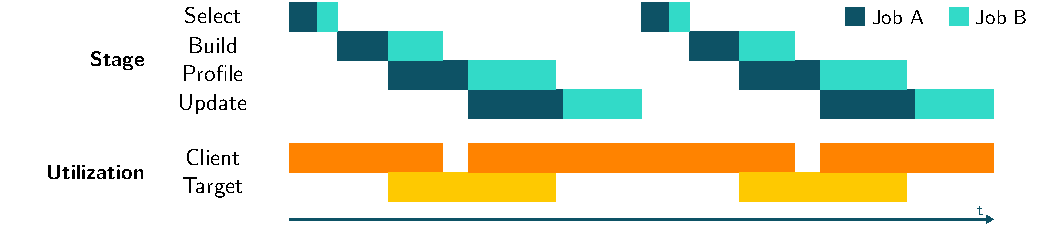
\includegraphics[width=\textwidth]{tvm_resource_utilization_interleaving}%
	\caption{Interleaving of multiple autotuning jobs}
	\label{fig:interleaving}
\end{figure}

Figure \ref{fig:interleaving} illustrates round-robin-based interleaving with an example of two jobs. Significant events are marked with numbers. Job A and Job B are started at the same time, but assume that the scheduler knows first about A. The first stage of A is executed, then the first stage of B. Once B finishes, the scheduler decides it is A's turn again and executes its second stage. Once A finishes the seconds stage, the client machine is free and B can execute the second stage. At the same time, A is ready to execute the third stage which will run on the target device. Since the target device is not in use, A can execute the profiling there in parallel to B's building since they use separate resources (\textbf{\textit{1}}). Building does not take as long as profiling, so A is ready to profile before B finishes its profiling stage. Therefore, A's third stage is postponed until the target device is free (\textbf{\textit{2}}). A's profiling and B's update model can, once again, execute simultaneously since they use distinct resources. After one iteration of all four stages, the process starts anew with the first stage (\textbf{\textit{3}}). This continues until both jobs are done. In a real scenario, new jobs might appear while other jobs are already running. The scheduler simply adds them to its list of jobs and includes them in the interleaving. Note how the resource utilization in Figure \ref{fig:interleaving} is much improved over the single-job autotuning in Figure \ref{fig:tvm-res-util} due to overlapping and sharing. Especially on the client device, utilization has almost been maximized since three of the four stages use the client.\todo{check if is consistent with new scheduler algorithm}

\subsection{Autotuning Decomposition}
The default autotuning process is monolithic and can be regarded as a blackbox from the outside (Figure \ref{fig:autotuning-decomposition-before}). This means, the autotuning loop can be started, and it does not finish until the whole job is completed. Once a stage finishes, the next one is executed immediately. However, the scheduler needs to be able to control the execution of the individual stages because it needs to prevent interference by means of delayed execution. This necessitates the decomposition of the autotuning process into schedulable units, corresponding to the stages  (Figure \ref{fig:autotuning-decomposition-after}). The client does not execute any of the stages on its own. Rather, it provides an interface to execute schedulable units and waits for an external trigger to do so. The autotuning loop can now run in another component, such as the scheduler.

\begin{figure}
	\begin{minipage}[b]{.5\textwidth}
		\centering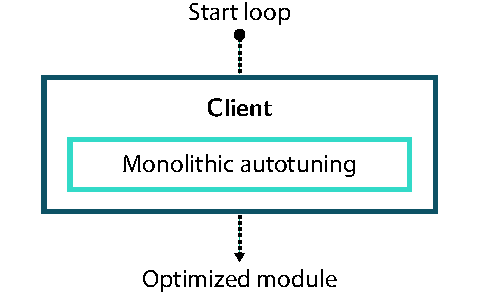
\includegraphics{autotuning_decomposition_before}
		\subcaption{Before decomposition}\label{fig:autotuning-decomposition-before}
	\end{minipage}%
	\begin{minipage}[b]{.5\textwidth}
		\centering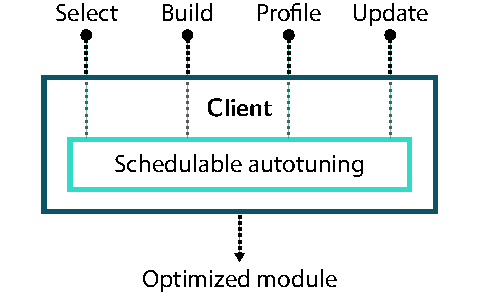
\includegraphics{autotuning_decomposition_after}
		\subcaption{After decomposition}\label{fig:autotuning-decomposition-after}
	\end{minipage}
	\caption{Client interface before and after decomposition}
	\label{fig:autotuning-decomposition}
\end{figure}

\subsection{Scheduling Algorithm}
To fulfill the task of interleaving while preventing interference, the scheduler needs to know four pieces of information for every job:
\begin{itemize}
	\item Whether the current stage is done; lets scheduler know if the job is ready for next stage
	\item Whether the whole job is done; lets scheduler know if the job needs to be considered in the future
	\item Which resource the current stage runs on; lets scheduler know which resources are free and which are in use
	\item Which resource the next stage will run on; lets scheduler postpone stage execution to prevent interference
\end{itemize}
We call this \textit{load-awareness}; being aware of the state of jobs and resources as well as their relationships. Theoretically, this allows the scheduler to work not only with TVM's autotuning but any process that can provide this information. Designing our scheduler to be agnostic of the underlying process also simplifies the algorithm.

In case multiple jobs are ready to execute a stage, the scheduler needs to decide which one to run. The simplest approach is to use a round-robin algorithm, which iterates over the jobs in the order they were started and picks the first one that is ready. More sophisticated approaches might apply some logic to decide on a job which would maximize resource utilization but keep the average autotuning time low. However, we choose the round-robin algorithm for our first version. It is easy to implement and works reasonably well for an arbitrary number of jobs, which allows us to proof our concept.

We present the algorithm for interleaved scheduling in Listing \ref{lst:sched-algo-interleaving}. Each job is controlled using an interface that provides the four pieces of information necessary for scheduling. The scheduler keeps a list of jobs in the order in which they were registered. Furthermore, it keeps a list of resources which are marked as free or busy. Each resource also has a queue which contains stages that are ready and will use that resource (Line 1). The algorithm is an infinite loop (Line 2), with each iteration consisting of two phases: scheduling and execution. In the first phase, the scheduler checks for each job if the current stage is done (Lines 4--5). Busy jobs are not regarded further. If the stage is done, the resource that was used is marked as free (Line 6). If the stage was the last stage in the job, the job can be removed from the list of jobs (Line 7--8). Otherwise, the job is ready to continue and the next stage is added to the queue of the resource that it will run on (Line 9--10). The iteration over all jobs in order is what effectively makes this round-robin scheduling. In the second phase, the scheduler iterates over each resource and the corresponding queue (Line 12). If the resource is free and there are pending stages for that resource, the first stage in the queue is dequeued and executed (Lines 13--15). The respective resource needs to be marked as busy (Line 16).

\begin{listing}
\begin{pythoncode}
queues = {r: [] for r in resources}
while True:
    # Phase 1: Round-robin scheduling
    for job in jobs:
        if job.is_stage_done():
            mark_as_free(job.previous_resource)
            if job.is_complete():
                jobs.remove(job)
            else:
                queues[job.next_resource].enqueue(job.next_stage)
    # Phase 2: Execution
    for resource, queue in queues:
        if is_free(resource) and len(queue) > 0:
            stage = queue.dequeue()
            stage.execute()
            mark_as_busy(resource)
\end{pythoncode}
\unskip
\caption{Interleaved scheduling pseudocode}
\label{lst:sched-algo-interleaving}
\end{listing}

Additionally to interleaving, our scheduler supports two other strategies for executing multiple jobs, which will be used in the evaluation for comparison.

Sequential scheduling (Listing \ref{lst:sched-algo-sequential}) works similar to single-job autotuning without a scheduler. Jobs do not run in parallel, but the next job is only started when the previous one finishes. This renders consideration of resource free/busy state unnecessary, and stages do not need to be postponed. However, since it is controlled by the scheduler, we can calculate the overhead introduced by adding a scheduler component, e.g., due to communication between scheduler and client or scheduling itself.

\begin{listing}
\begin{pythoncode}
while True:
    job = jobs.next()
    if not job:
        continue

    while not job.is_complete():
        if job.is_stage_done():
            job.next_stage.execute()
    jobs.remove(job)
\end{pythoncode}
\unskip
\caption{Sequential scheduling pseudocode}
\label{lst:sched-algo-sequential}
\end{listing}

Synchronous scheduling (Listing \ref{lst:sched-algo-synchronous}) forces parallel execution of the same stage of multiple jobs on the same resource, making it the exact opposite of interleaved scheduling. Postponed stage execution is applied here to guarantee full interference. We use this strategy to evaluate the worst case effect of interference. However, this only works for equal jobs, since there needs to be symmetry between stages of all jobs.

\begin{listing}
\begin{pythoncode}
while True:
    current_jobs = jobs
    if len(current_jobs) < 2:
        continue

    while not any([j.is_complete() for j in current_jobs]):
        if all([j.is_stage_done() for j in current_jobs]):
            [j.next_stage.execute() for j in current_jobs]
    jobs.remove_all(current_jobs)
\end{pythoncode}
\unskip
\caption{Synchronous scheduling pseudocode}
\label{lst:sched-algo-synchronous}
\end{listing}

\subsection{Autotuning Process}
\begin{figure}[ht]
	\centering
	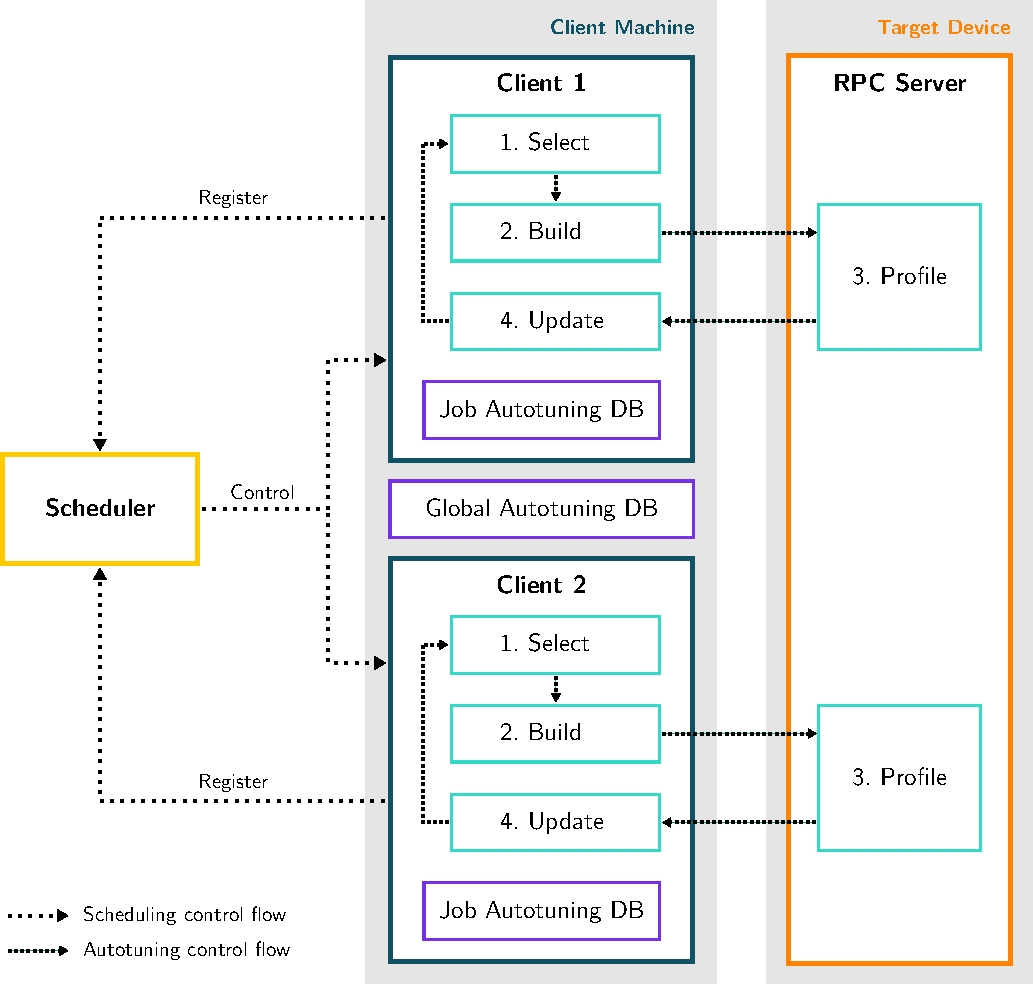
\includegraphics[width=\textwidth]{tvm_autotuning_with_scheduler.pdf}%
	\caption{Autotuning process with scheduler}
	\label{fig:tvm-autotuning-with-scheduler}
\end{figure}

Figure \ref{fig:tvm-autotuning-with-scheduler} shows the autotuning process with our scheduler (compare with scheduler-less, single-job autotuning in Figure \ref{fig:tvm-autotuning}). There are two discrete control flows at work. The per-job autotuning control flow is the same as before, spanning client and target machines. The scheduling control flow is on a higher level incorporating multiple jobs, and spans schedulers and clients. A new job needs to be made known to the scheduler first so it can consider the job in scheduling. One client is responsible for running exactly one job, registering that job with the scheduler when launching. The client is then ready to receive control commands to execute individual stages. The client exposes the interface which is required by the scheduling algorithm while calling the respective TVM methods internally. Clients can share target devices since the scheduler prevents interference of the profiling stages of multiple jobs on the same resource. The normal autotuning process is then executed, however not in one monolithic step, but stage for stage, enabled by the decomposition. Possibly there are some waiting times between stages introduces by postponing.

In multi-client scenarios, the cost model of each client is initialized by transfer learning from the global autotuning database on the client machine, which contains data from all jobs that have previously been executed on that machine. During autotuning, measurement results are written into a job-specific database which is merged back into the global database when the job is complete.

\section{Implementation}
Since TVM provides the API for autotuning in Python only, we use Python 3.6 for our implementation. It is intended as a proof of concept which we want to develop rapidly to see if the interleaving scheduler delivers the expected results. Therefore, we create an implementation that does not offer much flexibility or fault tolerance. However, it is sufficient to perform experiments in our test environment. The scheduler implementation is built on top of SimpleTVM for interfacing with TVM's autotuning.

For the beginning, only a single client machine is supported, but an arbitrary number of clients can run on it. Multiple target devices can be utilized for profiling, but the scheduler regards all target devices as a single resource. This coarse granularity is another decision to facilitate simple implementation.

\subsection{Components}
Show whole stack, denote what happens in scheduler, what happens in runner
Show which communication is in-process and which is RPC
JobManager negotiates between autotuning stages interface and simple scheduler interface, keeps track at position in autotuning
show abstract scheduler and client interface

\begin{figure}[ht]
	\centering
	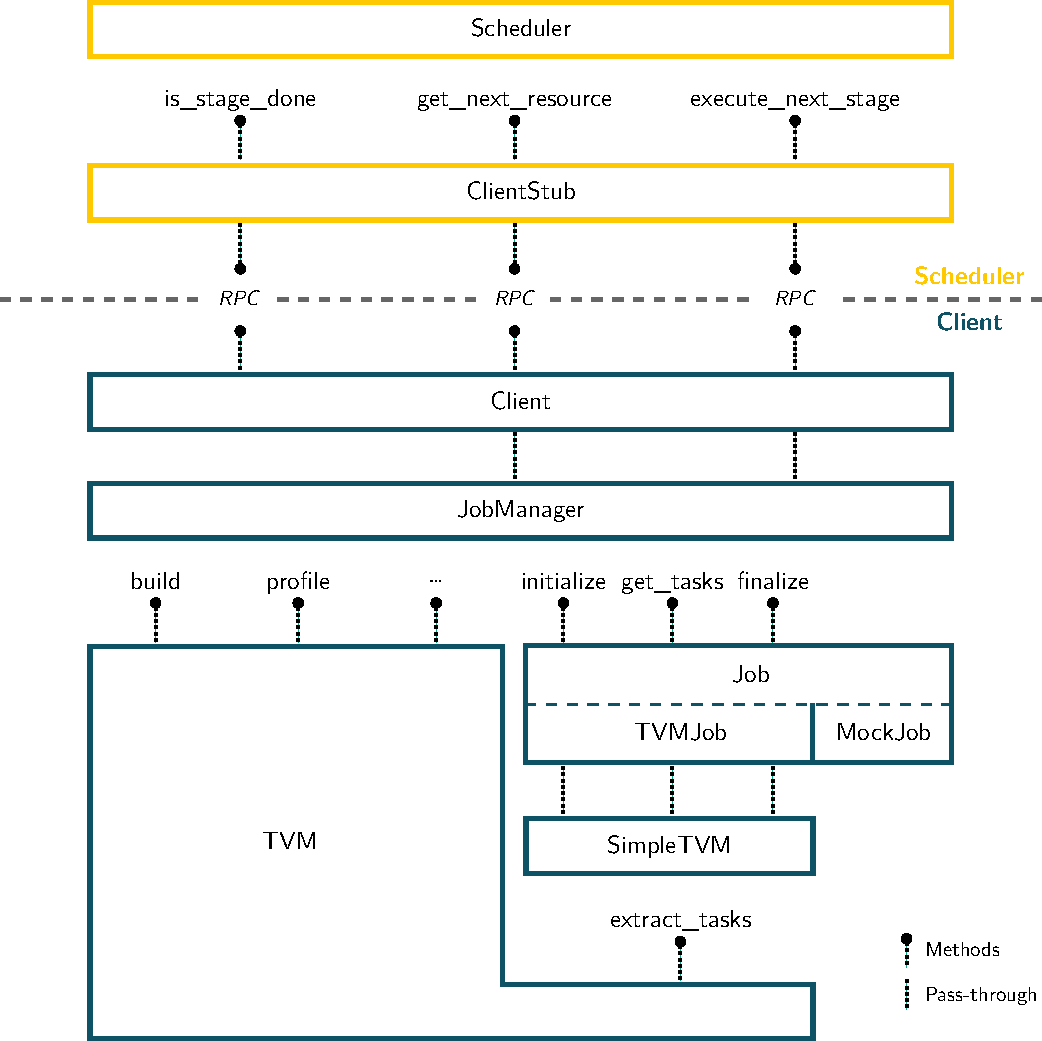
\includegraphics[width=\textwidth]{scheduler_layers}%
	\caption{Layers and components of scheduler implementation}
	\label{fig:scheduler_layers}
\end{figure}

\subsection{RPC}
Scheduler and clients live in different processes, usually even separate containers or physical servers. While the autotuning control flow already exists in form of in-process method calls and \gls{rpc} for remote profiling, the scheduling control flow requires its own \gls{rpc} infrastructure to enable communication between the scheduler and the clients. We create a simple HTTP-based \gls{rpc} protocol which supports exactly the interface required by scheduling.

Both scheduler and client act as HTTP server and client.

retry with exponential backoff

\subsection{Challenges}
initially wanted to run scheduler and clients in one multi-threaded process without RPC to get results quickly
not possible due to python global interpreter lock

evaluation of design choices takes long because autotuning is a slow process, created MockJob for debugging of scheduler

\section{Autotuning as a Service}
imagine autotuning as a service where users can submit their trained model and receive an optimized version according to SLA
Describe as a service
More sophisticated scheduler, requires moving more autotuning logic from client to scheduler
Make client stateless

Keep trained model and update it every n new entries to skip transfer learning time for every task
Check currently known best configurations and see if SLA is already met before actually starting autotuning
Automatically set up autotuning infrastructure
Split jobs on task and search space level to parallelize more
- make better use of unused resources
- faster autotuning, e.g. for paying customers